\section{Métodos de interpolación}
\label{sec:cap2-metodos-interpolacion}
La interpolación espacial, consiste en la utilización de puntos con valores conocidos, también
denominados puntos de control, para estimar el valor de una variable en lugares donde se
desconoce. Donde la estimación de los valores que alcanza una variable $Z$ en un conjunto de
puntos definidos por un par de coordenadas $(X,Y)$, partiendo de los valores de $Z$ medidos en
una muestra de puntos situados en el mismo área de estudio \citep{fAlonsoSig2006}.


Todos los métodos de interpolación se basan en la presunción lógica de que cuanto más cercanos
están dos puntos sobre la superficie terrestre, los valores de cualquier variable cuantitativa que
midamos en ellos serán más parecidos, para expresarlo más técnicamente, las variables espaciales
muestran autocorrelación espacial \citep{fAlonsoSig2006}.

El resultado de la interpolación espacial depende de un algoritmo computacional o una ecuación
matemática en la cual se emplean los datos de los puntos de control\cite{NINO2011}.


\subsection {Red de Triángulos Irregulares}
Las Redes Irregulares de Triángulos o TIN (por sus siglas en inglés Triangulated Irregular Network)
, se generan a partir de valores puntuales tratando de conseguir triángulos que maximicen la
relación área/perímetro, el conjunto de todos los triángulos forma un objeto geométrico
denominado conjunto convexo \citet{fAlonsoSig2006}.

\begin{figure}[H]
\centering
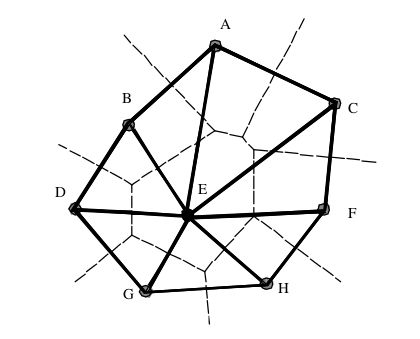
\includegraphics[width=0.4\textwidth]{capitulo-2/graphics/TIN-cPachecoMDE2003.png}
\caption{\label{fig:sig-tin}Red de Triángulos Irregulares (TIN) (Tomado de \cite{cPachecoMDE2003}).}
\end{figure}

TIN utiliza los puntos de entrada para construir una red de triángulos según el criterio de Delauny
\footnote{El criterio de Delauny genera, tanto como le es posible, triángulos pequeños y
equiláteros y es ley ser utilizado para crear objetos TIN}: en cada triángulo, el círculo que pasa
a través de los tres vértices no encierra ningún otro punto de entrada \citep{cPachecoMDE2003}.

\subsection{Ponderación de la inversa de la distancia}
Ponderación de la inversa de la distancia o IDW (por sus siglas en inglés Inverse distance
weighting), estima los puntos del modelo realizando una asignación de pesos a los datos del
entorno en función inversa a la distancia que los separa del punto en cuestión. De esta forma,
la influencia del valor observado $u_{i}$, sobre el valor estimado $u$, disminuye a medida que incrementa la distancia entre ambos.


\begin{figure}[H]
\centering
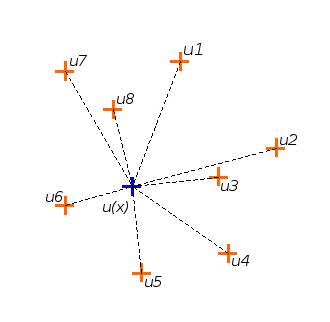
\includegraphics[width=0.5\textwidth]{capitulo-2/graphics/idw-distancia.jpg}
\caption{\label{fig:sig-idw-distancia}Cálculo de la distancia entre el punto a estimar,$u(x)$ , y los valores conocidos $u_{i}$.}

\end{figure}

La forma general de encontrar un valor interpolado $u$ en un punto $x$ basado en un conjunto de
muestras $u_i = u (x_i)$ para $i = 0,1, ..., N$ utilizando IDW es una función de interpolación:

\begin{equation}\label{eq:interpolacion-idw}
 u(x) = \sum_{i=1}^{N} w_i(X) * u_{i}
\end{equation}

Donde :

\begin{equation}
w_i(X) =  \dfrac{d(X, X_i)^{-p}}{\sum_{j=1}^{N} d(X, X_i)^{-p}}
\end{equation}


Siendo $d(X, X_i)$ una función que determina la distancia existente entre $X$ y $X_{i}$, donde $p$
es el exponente de ponderación. La elección del exponente de ponderación, $p$, determina la
contribución de los puntos circundantes al punto a interpolar, cuanto mayor es $p$, más
contribuyen los puntos próximos (\figref{fig:sig-idw-parametros}).

\begin{figure}[H]
\centering
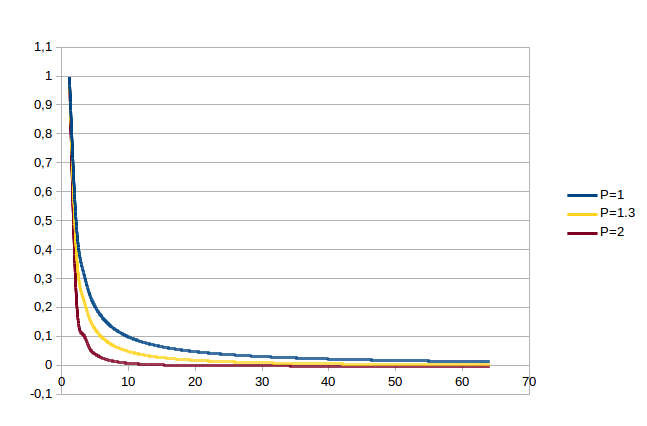
\includegraphics[width=0.8\textwidth]{capitulo-2/graphics/idw-parametros.png}
\caption{\label{fig:sig-idw-parametros} Nivel de influencia de distintos valores de $p$ en
relación a la distancia.}

\end{figure}

\subsection{Kriging}
El Kriging es un método geoestadístico de interpolación espacial de carácter global, exacto y
estocástico\citep{NINO2011}. El método cuantifica la estructura espacial de los datos, mediante el
uso de variogramas llamados algunas veces semivariogramas debido a su similitud en el cálculo, y
los predice \citep{villatoro2007comparacion}. La idea básica de este método corresponde a la
noción de dependencia espacial, según la cual las muestras cercanas tienen mayor similitud entre
sí que las más apartadas \citep{NINO2011}. El procedimiento analiza la variación estadística en
valores sobre diferentes distancias y diferentes direcciones determinando así la forma y el tamaño
del punto del área seleccionada y la serie de factores predominantes que pueden provocar el mínimo
error en la elevación estimada \citep{cPachecoMDE2003}.

La medición de la probabilidad, efectuada por los métodos del kriging, hace la diferencia con
respecto a los métodos determinísticos para interpolaciones espaciales
\citep{villatoro2007comparacion}.

Se presenta con un método de interpolación con una expresión general similar a la anterior, IDW,
con la diferencia básica es que asume que la altitud puede definirse como una variable
regionalizada.

\begin{equation}\label{eq:interpolacion-kriging}
 u(x) = \sum_{i=1}^{N} \lambda{i}(X) * u_{i}
\end{equation}

Donde $\lambda{i}(x)$ es el peso asignado al valor observado de $u_{i}$ y se puede calcular
resloviendo la siguiente ecuación :

\begin{equation}\label{eq:interpolacion-peso-kriging}
\sum_{i=1}^{N} \lambda{i}  * \gamma[d(X_{i}, X_{j})] + m = \gamma[d(X_{0}, X_{i})]
\end{equation}

Donde $m$ es el multiplicador de Lagrange utilizado para la minimización de las restricciones,
los subíndices $i$ y $j$ denotan a los puntos muestreados, el subíndice $0$ es el punto de
estimación, $\lambda$ es el peso dado a cada una de las observaciones y la suma de todos los
$\lambda$ es igual a uno y $d(X_{0}, X_{i})$ es la distancia entre $X_{i}$ y $X_{0}$ a partir del
semivariograma \citep{villatoro2007comparacion}:

\begin{equation}\label{eq:interpolacion-semivariograma}
\gamma[d(X_{i}, X_{0})] = var[z(X_{0} - z(X_{i}))]
\end{equation}

Esta semivarianza calculada es una medida para determinar la similitud entre observaciones, en
donde a mayor similitud, menor semivarianza \citep{villatoro2007comparacion}.
